\chapter{Classical Synchronization Problems}

\section{Introduction}

Classical synchronization problems are fundamental operating systems problems that demonstrate coordination, mutual exclusion, deadlock avoidance, starvation prevention, and resource sharing among concurrent processes and threads.

These problems frequently appear in Software Development Engineer (SDE) interviews because they test understanding of:

\begin{itemize}
\item Concurrency
\item Semaphores
\item Monitors
\item Mutexes
\item Condition Variables
\item Deadlocks
\item Thread Coordination
\end{itemize}

\section{Producer Consumer Problem}

\subsection{Problem Statement}

A producer generates data and places it into a shared buffer. A consumer removes data from the buffer.

Requirements:

\begin{itemize}
\item Producer must not insert into a full buffer.
\item Consumer must not remove from an empty buffer.
\item Shared buffer access must be synchronized.
\end{itemize}

\subsection{Visualization}

\begin{figure}[H]
\centering
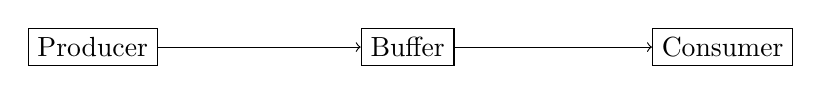
\begin{tikzpicture}
\node[draw] (p) at (0,0) {Producer};
\node[draw] (b) at (4,0) {Buffer};
\node[draw] (c) at (8,0) {Consumer};

\draw[->] (p)--(b);
\draw[->] (b)--(c);
\end{tikzpicture}
\caption{Producer Consumer Architecture}
\end{figure}

\subsection{Synchronization Challenges}

\begin{itemize}
\item Race conditions
\item Buffer overflow
\item Buffer underflow
\item Mutual exclusion
\end{itemize}

\subsection{Semaphore Solution}

Semaphores:

\begin{itemize}
\item mutex = 1
\item empty = N
\item full = 0
\end{itemize}

\begin{lstlisting}[language=C,style=interviewcode]
wait(empty);
wait(mutex);

insert_item();

signal(mutex);
signal(full);
\end{lstlisting}

\subsection{Monitor Solution}

\begin{lstlisting}[language=C++,style=interviewcode]
monitor Buffer {
condition notFull;
condition notEmpty;
}
\end{lstlisting}

\subsection{Modern Implementation}

\begin{itemize}
\item Java BlockingQueue
\item Go Channels
\item Python Queue
\item Message Brokers
\end{itemize}

\subsection{Complexity Discussion}

[
Time = O(1)
]

per insert/remove operation.

\subsection{Execution Example}

Producer inserts:

[
A,B,C
]

Consumer removes:

[
A \rightarrow B \rightarrow C
]

\subsection{C Example}

\begin{lstlisting}[language=C,style=interviewcode]
sem_wait(&empty);
sem_wait(&mutex);

buffer[in++] = item;

sem_post(&mutex);
sem_post(&full);
\end{lstlisting}

\subsection{Java Example}

\begin{lstlisting}[language=Java,style=interviewcode]
BlockingQueue<Integer> q =
new ArrayBlockingQueue<>(10);
\end{lstlisting}

\subsection{Python Example}

\begin{lstlisting}[language=Python,style=interviewcode]
from queue import Queue
q = Queue(10)
\end{lstlisting}

\subsection{Interview Follow-Up}

How would you support multiple producers and consumers?

\section{Bounded Buffer Problem}

\subsection{Problem Statement}

Producer Consumer with finite buffer size.

\subsection{Visualization}

\begin{figure}[H]
\centering
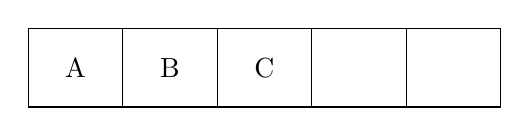
\begin{tikzpicture}

\draw (0,0) rectangle (6,1);

\draw (1.2,0)--(1.2,1);
\draw (2.4,0)--(2.4,1);
\draw (3.6,0)--(3.6,1);
\draw (4.8,0)--(4.8,1);

\node at (0.6,0.5) {A};
\node at (1.8,0.5) {B};
\node at (3,0.5) {C};

\end{tikzpicture}
\caption{Bounded Buffer}
\end{figure}

\subsection{Synchronization Challenges}

\begin{itemize}
\item Finite capacity
\item Concurrent access
\item Blocking conditions
\end{itemize}

\subsection{Semaphore Solution}

Identical to Producer Consumer using:

\begin{itemize}
\item mutex
\item full
\item empty
\end{itemize}

\subsection{Monitor Solution}

Use condition variables:

\begin{itemize}
\item notFull
\item notEmpty
\end{itemize}

\subsection{Modern Implementation}

Thread-safe queues and ring buffers.

\subsection{Complexity Discussion}

[
O(1)
]

for enqueue and dequeue.

\section{Readers Writers Problem}

\subsection{Problem Statement}

Multiple readers can read simultaneously.

Writers require exclusive access.

\subsection{Visualization}

\begin{figure}[H]
\centering
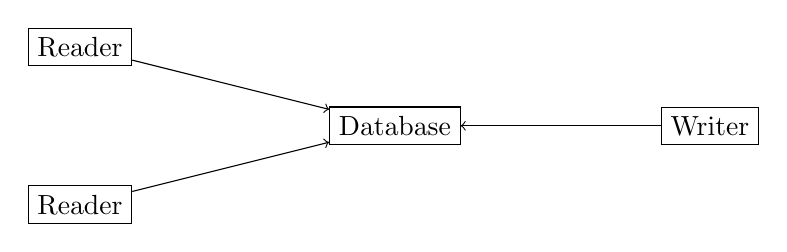
\begin{tikzpicture}

\node[draw] (r1) at (0,1) {Reader};

\node[draw] (r2) at (0,-1) {Reader};

\node[draw] (db) at (4,0) {Database};

\node[draw] (w) at (8,0) {Writer};

\draw[->] (r1)--(db);
\draw[->] (r2)--(db);
\draw[->] (w)--(db);

\end{tikzpicture}
\caption{Readers Writers Problem}
\end{figure}

\subsection{Synchronization Challenges}

\begin{itemize}
\item Reader starvation
\item Writer starvation
\item Fairness
\end{itemize}

\subsection{Semaphore Solution}

\begin{lstlisting}[language=C,style=interviewcode]
wait(mutex);
readCount++;
if(readCount == 1)
wait(rw_mutex);
signal(mutex);
\end{lstlisting}

\subsection{Monitor Solution}

Use:

\begin{itemize}
\item canRead
\item canWrite
\end{itemize}

condition variables.

\subsection{Modern Implementation}

\begin{itemize}
\item ReadWriteLock (Java)
\item shared_mutex (C++)
\end{itemize}

\subsection{Complexity Discussion}

[
O(1)
]

lock acquisition.

\subsection{Interview Follow-Up}

How would you eliminate writer starvation?

\section{Dining Philosophers Problem}

\subsection{Problem Statement}

Five philosophers share five chopsticks.

Each philosopher needs two chopsticks to eat.

\subsection{Visualization}

\begin{figure}[H]
\centering
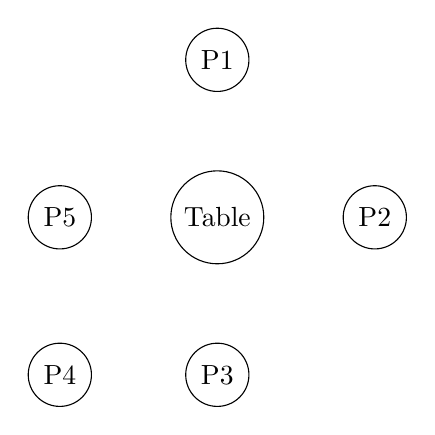
\begin{tikzpicture}
\node[draw,circle] (p1) at (0,2) {P1};
\node[draw,circle] (p2) at (2,0) {P2};
\node[draw,circle] (p3) at (0,-2) {P3};
\node[draw,circle] (p4) at (-2,-2) {P4};
\node[draw,circle] (p5) at (-2,0) {P5};

\node[draw,circle] at (0,0) {Table};
\end{tikzpicture}
\caption{Dining Philosophers}
\end{figure}

\subsection{Synchronization Challenges}

\begin{itemize}
\item Deadlock
\item Starvation
\item Resource contention
\end{itemize}

\subsection{Semaphore Solution}

Limit philosophers:

[
N-1
]

to eat simultaneously.

\subsection{Monitor Solution}

Monitor tracks fork states.

\subsection{Modern Implementation}

Lock ordering strategy.

\subsection{Complexity Discussion}

[
O(1)
]

resource acquisition.

\subsection{C Example}

\begin{lstlisting}[language=C,style=interviewcode]
wait(leftFork);
wait(rightFork);
eat();
signal(leftFork);
signal(rightFork);
\end{lstlisting}

\subsection{Interview Follow-Up}

How do you prevent deadlock?

\section{Sleeping Barber Problem}

\subsection{Problem Statement}

A barber sleeps when no customers exist.

Customers either:

\begin{itemize}
\item Get haircut
\item Wait
\item Leave
\end{itemize}

\subsection{Visualization}

\begin{figure}[H]
\centering
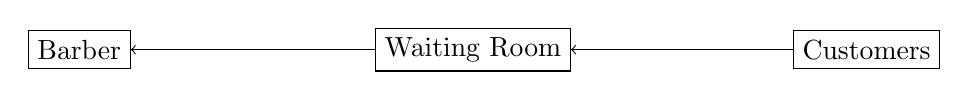
\begin{tikzpicture}

\node[draw] (b) at (0,0) {Barber};

\node[draw] (w) at (5,0) {Waiting Room};

\node[draw] (c) at (10,0) {Customers};

\draw[->] (c)--(w);
\draw[->] (w)--(b);

\end{tikzpicture}
\caption{Sleeping Barber}
\end{figure}

\subsection{Synchronization Challenges}

\begin{itemize}
\item Limited waiting chairs
\item Barber sleep/wakeup
\item Customer coordination
\end{itemize}

\subsection{Semaphore Solution}

Use:

\begin{itemize}
\item customers
\item barber
\item mutex
\end{itemize}

\subsection{Monitor Solution}

Condition variables manage waiting room.

\subsection{Modern Implementation}

Task queues and worker pools.

\subsection{Complexity Discussion}

[
O(1)
]

per customer.

\section{Cigarette Smokers Problem}

\subsection{Problem Statement}

Three smokers each possess one ingredient.

Agent supplies two ingredients.

Only the smoker with the missing ingredient can smoke.

\subsection{Visualization}

\begin{center}
Tobacco + Paper $\rightarrow$ Smoker with Matches
\end{center}

\subsection{Synchronization Challenges}

\begin{itemize}
\item Resource matching
\item Wakeup coordination
\end{itemize}

\subsection{Semaphore Solution}

Separate semaphores for each smoker.

\subsection{Monitor Solution}

Condition variables signal correct smoker.

\subsection{Modern Implementation}

Event-driven signaling.

\subsection{Complexity Discussion}

[
O(1)
]

selection.

\section{River Crossing Problem}

\subsection{Problem Statement}

Hackers and serfs must cross a river.

Boat capacity:

[
4
]

Unsafe combinations are disallowed.

\subsection{Visualization}

\begin{figure}[H]
\centering
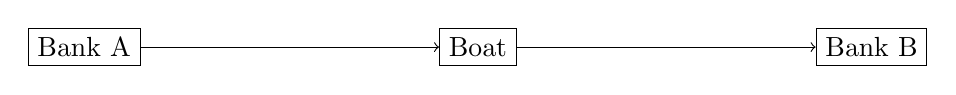
\begin{tikzpicture}

\node[draw] (left) at (0,0) {Bank A};

\node[draw] (boat) at (5,0) {Boat};

\node[draw] (right) at (10,0) {Bank B};

\draw[->] (left)--(boat);
\draw[->] (boat)--(right);

\end{tikzpicture}
\caption{River Crossing Problem}
\end{figure}

\subsection{Synchronization Challenges}

\begin{itemize}
\item Group formation
\item Safety constraints
\end{itemize}

\subsection{Semaphore Solution}

Counters plus semaphores coordinate boarding.

\subsection{Monitor Solution}

Monitor validates safe combinations.

\subsection{Modern Implementation}

Barrier plus locks.

\subsection{Complexity Discussion}

[
O(1)
]

coordination decisions.

\section{Barrier Synchronization Problem}

\subsection{Problem Statement}

All threads must reach a barrier before any proceed.

\subsection{Visualization}

\begin{figure}[H]
\centering
\begin{tikzpicture}

\node at (0,2) {T1};
\node at (0,1) {T2};
\node at (0,0) {T3};

\draw[thick] (4,-1)--(4,3);

\node[right] at (4,2) {Barrier};

\end{tikzpicture}
\caption{Barrier Synchronization}
\end{figure}

\subsection{Synchronization Challenges}

\begin{itemize}
\item Waiting for all threads
\item Reusable barriers
\end{itemize}

\subsection{Semaphore Solution}

Use:

\begin{itemize}
\item count
\item mutex
\item barrier semaphore
\end{itemize}

\subsection{Monitor Solution}

Condition variable waits until count reaches threshold.

\subsection{Modern Implementation}

\begin{itemize}
\item pthread_barrier
\item CyclicBarrier
\item CountDownLatch
\end{itemize}

\subsection{Complexity Discussion}

[
O(1)
]

per arrival.

\subsection{Java Example}

\begin{lstlisting}[language=Java,style=interviewcode]
CyclicBarrier barrier =
new CyclicBarrier(4);
\end{lstlisting}

\subsection{Python Example}

\begin{lstlisting}[language=Python,style=interviewcode]
from threading import Barrier
b = Barrier(4)
\end{lstlisting}

\section{Key Takeaways}

\begin{keytakeaways}
Classical synchronization problems illustrate fundamental concurrency concepts. Producer Consumer demonstrates buffer coordination. Readers Writers focuses on concurrent reads and exclusive writes. Dining Philosophers explores deadlock prevention. Sleeping Barber models waiting queues. Cigarette Smokers demonstrates selective signaling. River Crossing introduces group synchronization constraints. Barrier Synchronization ensures coordinated progress across threads. These problems form the foundation of modern concurrent system design.
\end{keytakeaways}

\section{Interview Questions with Answers}

\begin{enumerate}
\item What is the Producer Consumer problem?\
Shared buffer synchronization problem.

\item What causes buffer overflow?\
Producer inserting into a full buffer.

\item What causes buffer underflow?\
Consumer removing from an empty buffer.

\item Which semaphores are used in Producer Consumer?\
mutex, empty, full.

\item What is the Bounded Buffer problem?\
Producer Consumer with finite capacity.

\item What is the Readers Writers problem?\
Concurrent readers and exclusive writers.

\item Why can writers starve?\
Continuous reader arrivals.

\item What is a Read-Write lock?\
Lock supporting concurrent readers.

\item What is the Dining Philosophers problem?\
Resource allocation and deadlock problem.

\item How is deadlock prevented?\
Resource ordering or limiting access.

\item What is starvation?\
Indefinite waiting.

\item What is the Sleeping Barber problem?\
Synchronization with finite waiting room.

\item Why does the barber sleep?\
No waiting customers.

\item What is the Cigarette Smokers problem?\
Selective resource signaling problem.

\item What does the agent do?\
Provides two ingredients.

\item What is the River Crossing problem?\
Safe group coordination problem.

\item What is Barrier Synchronization?\
Threads wait for each other.

\item Modern barrier example?\
CyclicBarrier.

\item Monitor vs Semaphore?\
Monitor is higher-level abstraction.

\item Why are these problems important?\
They model real-world concurrency.

\item Which problem demonstrates fairness?\
Readers Writers.

\item Which problem demonstrates deadlock?\
Dining Philosophers.

\item Which problem demonstrates queue management?\
Sleeping Barber.

\item Which problem demonstrates event signaling?\
Cigarette Smokers.

\item Which problem demonstrates collective coordination?\
Barrier Synchronization.
\end{enumerate}

\section{MCQs with Answers}

\begin{enumerate}
\item Producer Consumer uses:
\begin{enumerate}[label=(\alph*)]
\item Cache
\item Shared Buffer
\item DMA
\item Paging
\end{enumerate}
Answer: (b)

\item Producer waits on:
\begin{enumerate}[label=(\alph*)]
\item full
\item empty
\item mutex only
\item none
\end{enumerate}
Answer: (b)

\item Consumer waits on:
\begin{enumerate}[label=(\alph*)]
\item full
\item cache
\item disk
\item CPU
\end{enumerate}
Answer: (a)

\item Readers Writers allows:
\begin{enumerate}[label=(\alph*)]
\item Multiple Readers
\item Multiple Writers
\item Infinite Writers
\item No Readers
\end{enumerate}
Answer: (a)

\item Writers require:
\begin{enumerate}[label=(\alph*)]
\item Shared Access
\item Exclusive Access
\item DMA
\item Cache
\end{enumerate}
Answer: (b)

\item Dining Philosophers demonstrates:
\begin{enumerate}[label=(\alph*)]
\item Deadlock
\item Paging
\item Scheduling
\item Caching
\end{enumerate}
Answer: (a)

\item Number of philosophers:
\begin{enumerate}[label=(\alph*)]
\item 2
\item 3
\item 5
\item 10
\end{enumerate}
Answer: (c)

\item Sleeping Barber includes:
\begin{enumerate}[label=(\alph*)]
\item Waiting Room
\item Cache
\item MMU
\item DMA
\end{enumerate}
Answer: (a)

\item Cigarette Smokers uses:
\begin{enumerate}[label=(\alph*)]
\item Ingredients
\item Pages
\item Frames
\item Segments
\end{enumerate}
Answer: (a)

\item River Crossing focuses on:
\begin{enumerate}[label=(\alph*)]
\item Group Safety
\item Memory
\item Files
\item CPU
\end{enumerate}
Answer: (a)

\item Barrier synchronization waits for:
\begin{enumerate}[label=(\alph*)]
\item All Threads
\item One Thread
\item Disk
\item Cache
\end{enumerate}
Answer: (a)

\item CyclicBarrier belongs to:
\begin{enumerate}[label=(\alph*)]
\item Java
\item C
\item SQL
\item Linux Shell
\end{enumerate}
Answer: (a)

\item Monitor provides:
\begin{enumerate}[label=(\alph*)]
\item High-Level Synchronization
\item Paging
\item Caching
\item DMA
\end{enumerate}
Answer: (a)

\item Semaphore is used for:
\begin{enumerate}[label=(\alph*)]
\item Synchronization
\item Compilation
\item Parsing
\item Linking
\end{enumerate}
Answer: (a)

\item Deadlock means:
\begin{enumerate}[label=(\alph*)]
\item Circular Waiting
\item Scheduling
\item Paging
\item Caching
\end{enumerate}
Answer: (a)

\item Starvation means:
\begin{enumerate}[label=(\alph*)]
\item Infinite Wait
\item Fast Execution
\item Paging
\item DMA
\end{enumerate}
Answer: (a)

\item Bounded Buffer size is:
\begin{enumerate}[label=(\alph*)]
\item Finite
\item Infinite
\item Zero
\item Dynamic Only
\end{enumerate}
Answer: (a)

\item ReadWriteLock solves:
\begin{enumerate}[label=(\alph*)]
\item Readers Writers
\item Barber
\item Smokers
\item River Crossing
\end{enumerate}
Answer: (a)

\item Queue is central to:
\begin{enumerate}[label=(\alph*)]
\item Producer Consumer
\item Segmentation
\item Paging
\item Caching
\end{enumerate}
Answer: (a)

\item Barrier ensures:
\begin{enumerate}[label=(\alph*)]
\item Coordinated Progress
\item Disk Access
\item Memory Allocation
\item Scheduling
\end{enumerate}
Answer: (a)

\item Mutex primarily provides:
\begin{enumerate}[label=(\alph*)]
\item Mutual Exclusion
\item Paging
\item DMA
\item Virtual Memory
\end{enumerate}
Answer: (a)

\item Semaphore value can:
\begin{enumerate}[label=(\alph*)]
\item Change
\item Never Change
\item Only Increase
\item Only Decrease
\end{enumerate}
Answer: (a)

\item Dining Philosophers use:
\begin{enumerate}[label=(\alph*)]
\item Chopsticks
\item Buffers
\item Pages
\item Queues
\end{enumerate}
Answer: (a)

\item Sleeping Barber models:
\begin{enumerate}[label=(\alph*)]
\item Service Queue
\item Paging
\item Swapping
\item MMU
\end{enumerate}
Answer: (a)

\item Barrier is an example of:
\begin{enumerate}[label=(\alph*)]
\item Collective Synchronization
\item Paging
\item Segmentation
\item Swapping
\end{enumerate}
Answer: (a)
\end{enumerate}

\section{Revision Notes}

\begin{revisionnotes}
\item Producer Consumer uses mutex, empty, full semaphores.
\item Bounded Buffer has finite capacity.
\item Readers Writers permits concurrent readers.
\item Writers require exclusive access.
\item Dining Philosophers demonstrates deadlock risks.
\item Sleeping Barber demonstrates waiting-room synchronization.
\item Cigarette Smokers demonstrates selective signaling.
\item River Crossing demonstrates safe group formation.
\item Barrier Synchronization coordinates thread progress.
\item Monitors are higher-level synchronization constructs.
\item Condition variables are used inside monitors.
\item Java provides BlockingQueue and CyclicBarrier.
\item Python provides Queue and Barrier.
\item Fairness prevents starvation.
\item Resource ordering prevents deadlock.
\end{revisionnotes}

\section{Cheat Sheet}

\begin{longtable}{|p{5cm}|p{8cm}|}
\hline
Problem & Core Concept \
\hline
Producer Consumer & Shared Buffer \
\hline
Bounded Buffer & Finite Capacity Queue \
\hline
Readers Writers & Read Sharing / Write Exclusivity \
\hline
Dining Philosophers & Deadlock Prevention \
\hline
Sleeping Barber & Waiting Room Synchronization \
\hline
Cigarette Smokers & Selective Resource Signaling \
\hline
River Crossing & Safe Group Formation \
\hline
Barrier Synchronization & Collective Progress \
\hline
Mutex & Mutual Exclusion \
\hline
Semaphore & Synchronization Primitive \
\hline
Monitor & High-Level Synchronization \
\hline
Condition Variable & Wait/Signal Mechanism \
\hline
Starvation & Infinite Waiting \
\hline
Deadlock & Circular Waiting \
\hline
Fairness & Guaranteed Access \
\hline
\end{longtable}
